% Options for packages loaded elsewhere
\PassOptionsToPackage{unicode}{hyperref}
\PassOptionsToPackage{hyphens}{url}
%
\documentclass[
]{article}
\usepackage{amsmath,amssymb}
\usepackage{lmodern}
\usepackage{iftex}
\ifPDFTeX
  \usepackage[T1]{fontenc}
  \usepackage[utf8]{inputenc}
  \usepackage{textcomp} % provide euro and other symbols
\else % if luatex or xetex
  \usepackage{unicode-math}
  \defaultfontfeatures{Scale=MatchLowercase}
  \defaultfontfeatures[\rmfamily]{Ligatures=TeX,Scale=1}
\fi
% Use upquote if available, for straight quotes in verbatim environments
\IfFileExists{upquote.sty}{\usepackage{upquote}}{}
\IfFileExists{microtype.sty}{% use microtype if available
  \usepackage[]{microtype}
  \UseMicrotypeSet[protrusion]{basicmath} % disable protrusion for tt fonts
}{}
\makeatletter
\@ifundefined{KOMAClassName}{% if non-KOMA class
  \IfFileExists{parskip.sty}{%
    \usepackage{parskip}
  }{% else
    \setlength{\parindent}{0pt}
    \setlength{\parskip}{6pt plus 2pt minus 1pt}}
}{% if KOMA class
  \KOMAoptions{parskip=half}}
\makeatother
\usepackage{xcolor}
\IfFileExists{xurl.sty}{\usepackage{xurl}}{} % add URL line breaks if available
\IfFileExists{bookmark.sty}{\usepackage{bookmark}}{\usepackage{hyperref}}
\hypersetup{
  pdftitle={American Samoa Model Checks},
  pdfauthor={Meg Oshima},
  hidelinks,
  pdfcreator={LaTeX via pandoc}}
\urlstyle{same} % disable monospaced font for URLs
\usepackage[margin=1in]{geometry}
\usepackage{graphicx}
\makeatletter
\def\maxwidth{\ifdim\Gin@nat@width>\linewidth\linewidth\else\Gin@nat@width\fi}
\def\maxheight{\ifdim\Gin@nat@height>\textheight\textheight\else\Gin@nat@height\fi}
\makeatother
% Scale images if necessary, so that they will not overflow the page
% margins by default, and it is still possible to overwrite the defaults
% using explicit options in \includegraphics[width, height, ...]{}
\setkeys{Gin}{width=\maxwidth,height=\maxheight,keepaspectratio}
% Set default figure placement to htbp
\makeatletter
\def\fps@figure{htbp}
\makeatother
\setlength{\emergencystretch}{3em} % prevent overfull lines
\providecommand{\tightlist}{%
  \setlength{\itemsep}{0pt}\setlength{\parskip}{0pt}}
\setcounter{secnumdepth}{-\maxdimen} % remove section numbering
\usepackage{amsmath}
\usepackage{booktabs}
\usepackage{caption}
\usepackage{longtable}
\ifLuaTeX
  \usepackage{selnolig}  % disable illegal ligatures
\fi

\title{American Samoa Model Checks}
\author{Meg Oshima}
\date{2022-08-19}

\begin{document}
\maketitle

\textbf{This is a summary report for the APRU base model run.}

\hypertarget{model-output}{%
\section{Model Output}\label{model-output}}

\hypertarget{input-data}{%
\subsection{Input Data}\label{input-data}}

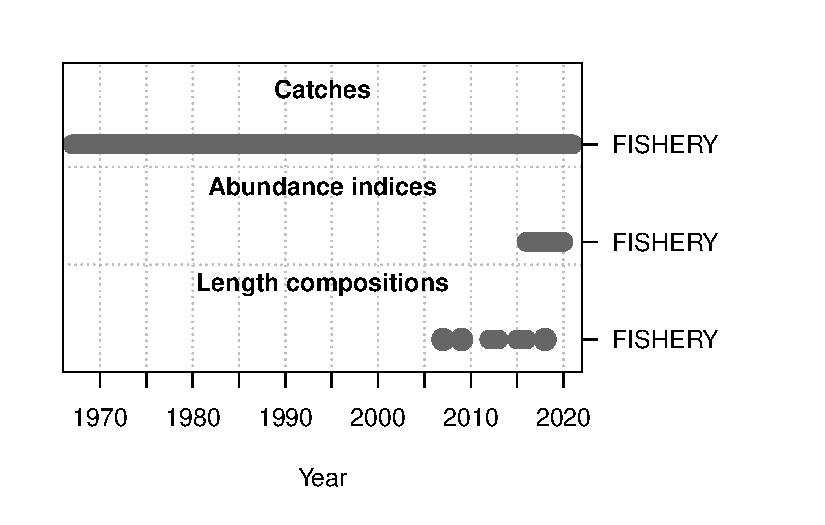
\includegraphics{C:/Users/Megumi.Oshima/Documents/AmSam-Bottomfish-2023/SS3 models/APRU/test_initf/0_APRU_test_initf_SS3_Diags_Report_files/figure-latex/unnamed-chunk-2-1.pdf}
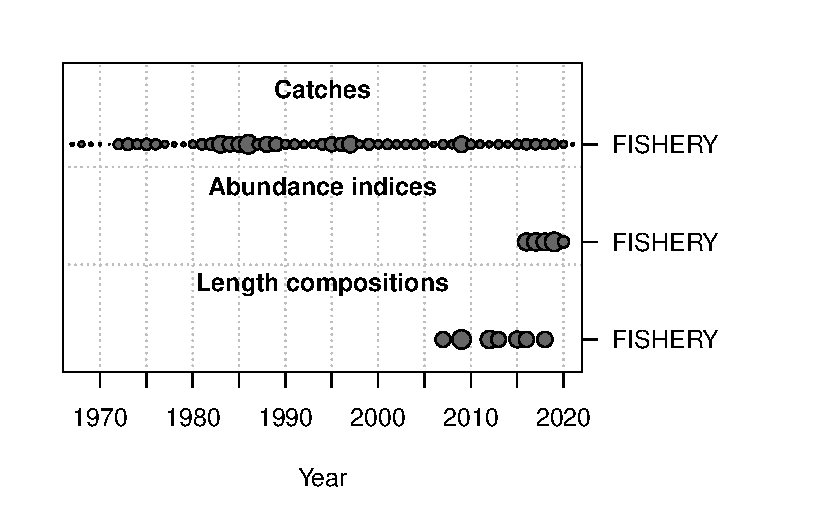
\includegraphics{C:/Users/Megumi.Oshima/Documents/AmSam-Bottomfish-2023/SS3 models/APRU/test_initf/0_APRU_test_initf_SS3_Diags_Report_files/figure-latex/unnamed-chunk-2-2.pdf}

\hypertarget{convergence-check}{%
\subsection{Convergence Check}\label{convergence-check}}

\begin{verbatim}
##   Converged     MaxGrad
## 1      TRUE 8.58368e-06
\end{verbatim}

\begin{verbatim}
## [1] "1 NOTE:  Max data length bin: 90  < max pop len bins: 100; so will accumulate larger pop len bins"
## [2] "N warnings: 1"
\end{verbatim}

\hypertarget{fit-to-model}{%
\subsection{Fit to Model}\label{fit-to-model}}

\hypertarget{cpue}{%
\subsubsection{CPUE}\label{cpue}}

\begin{center}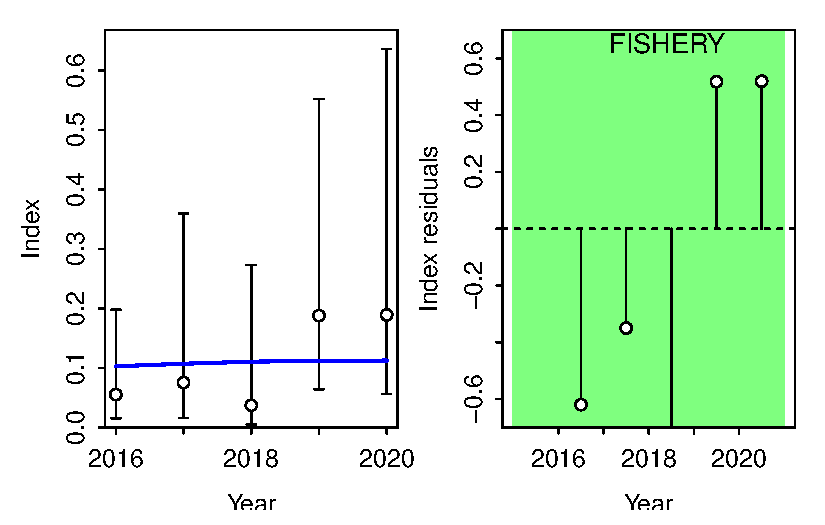
\includegraphics[width=.49\linewidth]{C:\Users\Megumi.Oshima\Documents\AmSam-Bottomfish-2023\SS3 models\APRU\test_initf\0_APRU_test_initf_SS3_Diags_Report_files/figure-latex/unnamed-chunk-4-1} \end{center}

\begin{verbatim}
## Residual Runs Test (/w plot) stats by Index:
\end{verbatim}

\begin{verbatim}
## Warning in simpleLoess(y, x, w, span, degree = degree, parametric = parametric, : Chernobyl! trL>n 6

## Warning in simpleLoess(y, x, w, span, degree = degree, parametric = parametric, : Chernobyl! trL>n 6
\end{verbatim}

\begin{verbatim}
## Warning in sqrt(sum.squares/one.delta): NaNs produced
\end{verbatim}

\begin{center}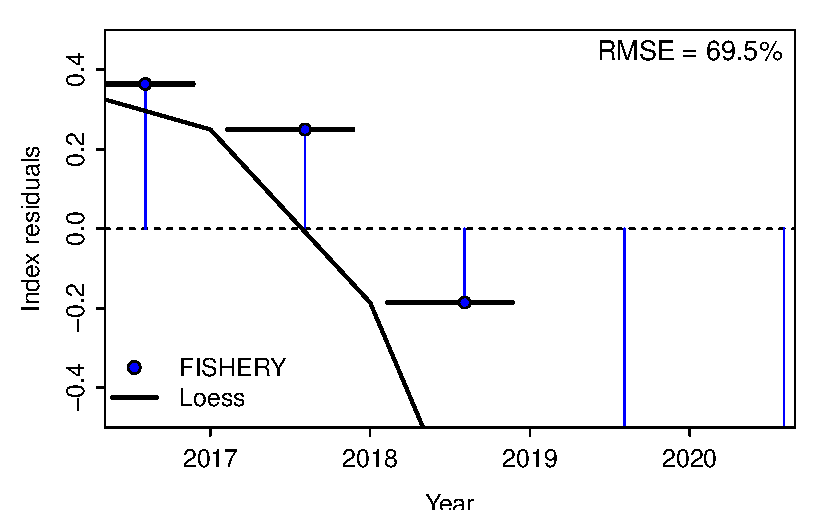
\includegraphics[width=.49\linewidth]{C:\Users\Megumi.Oshima\Documents\AmSam-Bottomfish-2023\SS3 models\APRU\test_initf\0_APRU_test_initf_SS3_Diags_Report_files/figure-latex/unnamed-chunk-4-2} \end{center}

\begin{verbatim}
## RMSE stats by Index:
\end{verbatim}

\hypertarget{length-comp}{%
\subsubsection{Length Comp}\label{length-comp}}

\captionsetup[table]{labelformat=empty,skip=1pt}
\begin{longtable}{rrrll}
\toprule
\#Factor & Fleet & New\_Var\_adj & Type & Name \\ 
\midrule
4 & 1 & 0.348222 & len & FISHERY \\ 
\bottomrule
\end{longtable}

\begin{verbatim}
## Residual Runs Test (/w plot) stats by Mean length:
\end{verbatim}

\begin{verbatim}
##     Index runs.p   test  sigma3.lo sigma3.hi type
## 1 FISHERY  0.623 Passed -0.1384455 0.1384455  len
\end{verbatim}

\begin{center}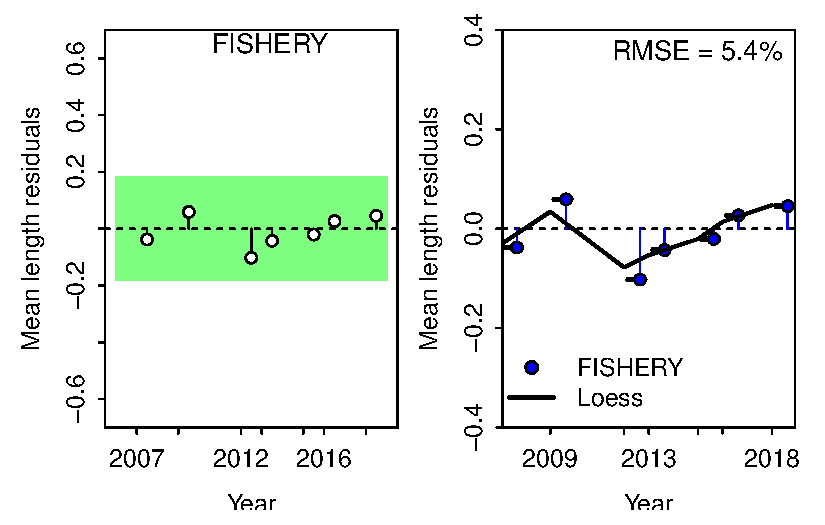
\includegraphics[width=.49\linewidth]{C:\Users\Megumi.Oshima\Documents\AmSam-Bottomfish-2023\SS3 models\APRU\test_initf\0_APRU_test_initf_SS3_Diags_Report_files/figure-latex/unnamed-chunk-5-1} \end{center}

\begin{verbatim}
## RMSE stats by Index:
\end{verbatim}

\begin{verbatim}
## # A tibble: 2 x 3
##   Fleet    RMSE.perc  Nobs
##   <chr>        <dbl> <int>
## 1 FISHERY        4.4    13
## 2 Combined       4.4    13
\end{verbatim}

\begin{center}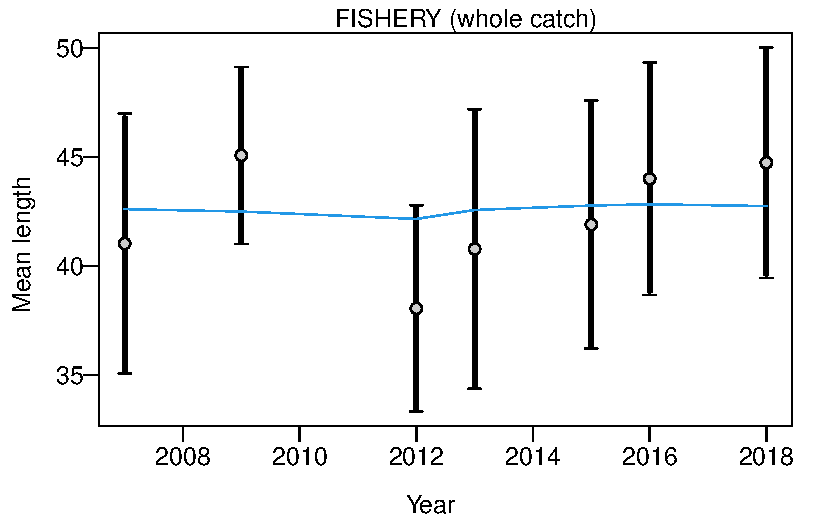
\includegraphics{C:\Users\Megumi.Oshima\Documents\AmSam-Bottomfish-2023\SS3 models\APRU\test_initf\0_APRU_test_initf_SS3_Diags_Report_files/figure-latex/unnamed-chunk-6-1} \end{center}

\begin{center}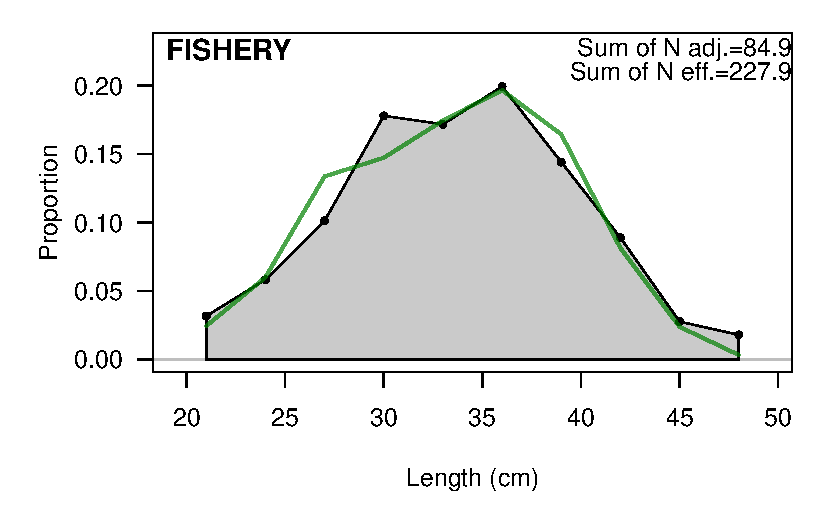
\includegraphics{C:\Users\Megumi.Oshima\Documents\AmSam-Bottomfish-2023\SS3 models\APRU\test_initf\0_APRU_test_initf_SS3_Diags_Report_files/figure-latex/unnamed-chunk-6-2} \end{center}

\begin{center}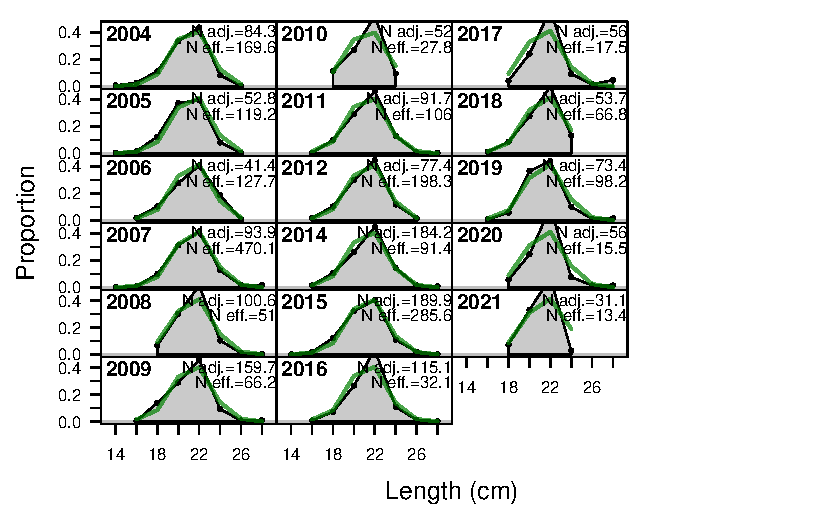
\includegraphics{C:\Users\Megumi.Oshima\Documents\AmSam-Bottomfish-2023\SS3 models\APRU\test_initf\0_APRU_test_initf_SS3_Diags_Report_files/figure-latex/unnamed-chunk-6-3} \end{center}

\hypertarget{retrospective-and-hindcasting}{%
\subsection{Retrospective and
Hindcasting}\label{retrospective-and-hindcasting}}

\hypertarget{retrospective}{%
\subsubsection{Retrospective}\label{retrospective}}

\begin{verbatim}
## [1] "No retrospective runs were found"
\end{verbatim}

\hypertarget{hindcasting}{%
\subsubsection{Hindcasting}\label{hindcasting}}

\begin{verbatim}
## [1] "No information for hindcast was found"
\end{verbatim}

\hypertarget{recruitment-deviations}{%
\subsection{Recruitment Deviations}\label{recruitment-deviations}}

\begin{verbatim}
## Skipped SSplotrecdevs - no rec devs estimated
\end{verbatim}

\hypertarget{likelihood-profile}{%
\subsection{Likelihood Profile}\label{likelihood-profile}}

\begin{verbatim}
## [1] "No likelihood runs were found"
\end{verbatim}

\hypertarget{management-quantities}{%
\subsection{Management Quantities}\label{management-quantities}}

\begin{verbatim}
## 
##  starter.sso with Bratio: SSB/SSBMSY and F: _abs_F 
## 
\end{verbatim}

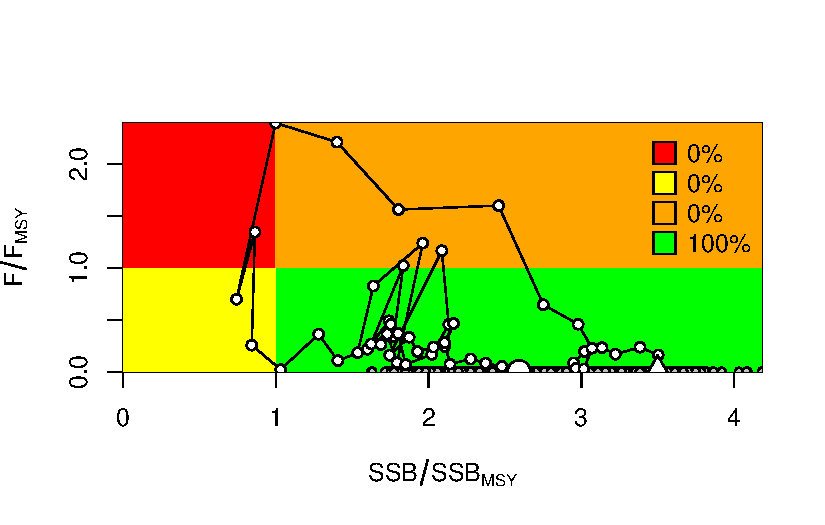
\includegraphics{C:/Users/Megumi.Oshima/Documents/AmSam-Bottomfish-2023/SS3 models/APRU/test_initf/0_APRU_test_initf_SS3_Diags_Report_files/figure-latex/unnamed-chunk-11-1.pdf}

\begin{verbatim}
## Plot Comparison of stock
\end{verbatim}

\begin{verbatim}
## Plot Comparison of harvest
\end{verbatim}

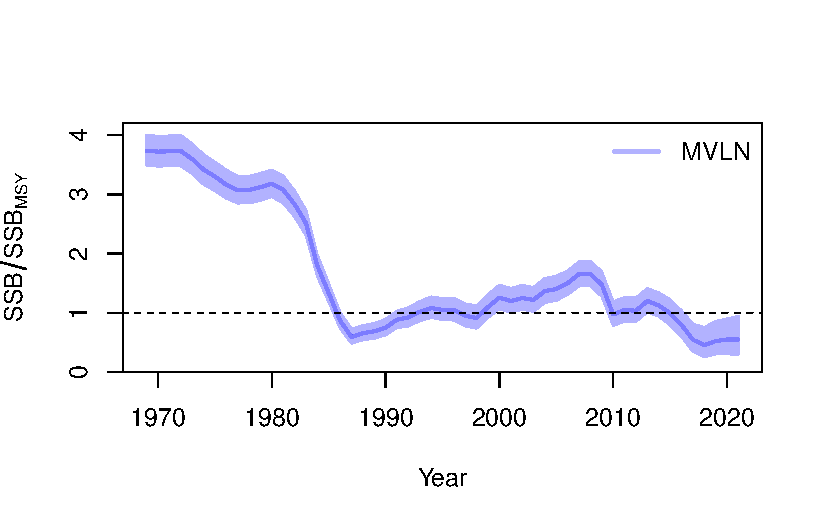
\includegraphics{C:/Users/Megumi.Oshima/Documents/AmSam-Bottomfish-2023/SS3 models/APRU/test_initf/0_APRU_test_initf_SS3_Diags_Report_files/figure-latex/unnamed-chunk-11-2.pdf}

\begin{verbatim}
## Plot Comparison of SSB
\end{verbatim}

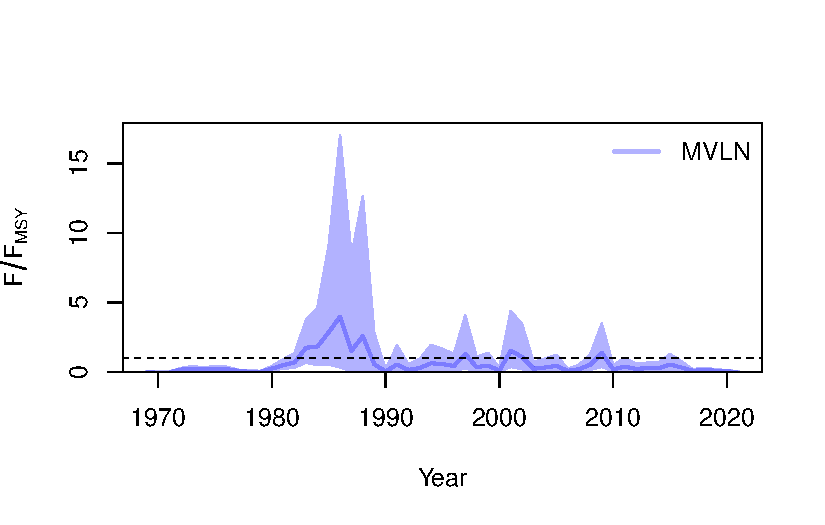
\includegraphics{C:/Users/Megumi.Oshima/Documents/AmSam-Bottomfish-2023/SS3 models/APRU/test_initf/0_APRU_test_initf_SS3_Diags_Report_files/figure-latex/unnamed-chunk-11-3.pdf}

\begin{verbatim}
## Plot Comparison of F
\end{verbatim}

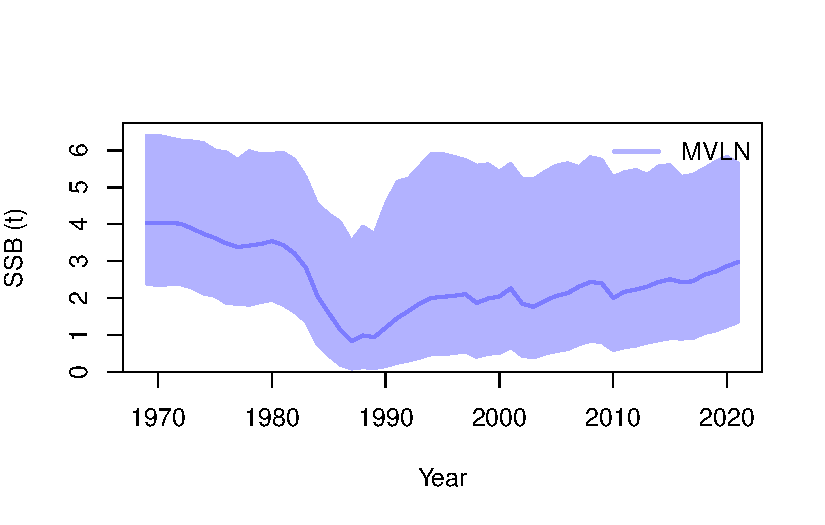
\includegraphics{C:/Users/Megumi.Oshima/Documents/AmSam-Bottomfish-2023/SS3 models/APRU/test_initf/0_APRU_test_initf_SS3_Diags_Report_files/figure-latex/unnamed-chunk-11-4.pdf}
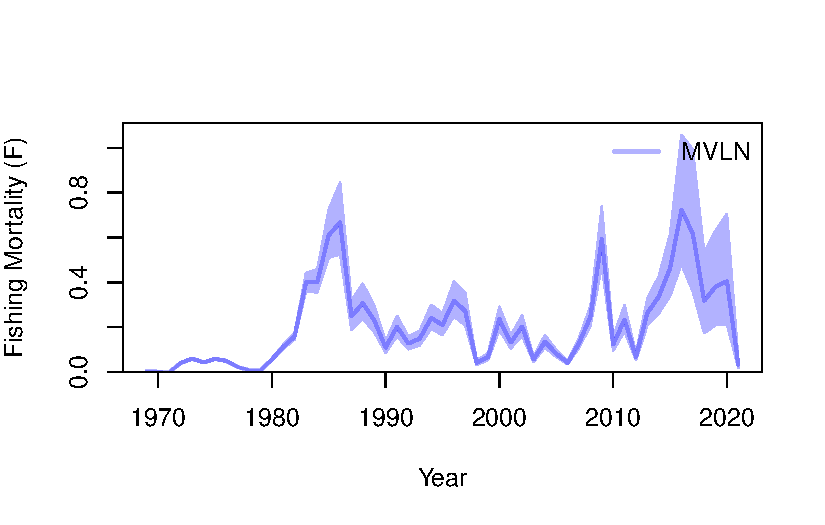
\includegraphics{C:/Users/Megumi.Oshima/Documents/AmSam-Bottomfish-2023/SS3 models/APRU/test_initf/0_APRU_test_initf_SS3_Diags_Report_files/figure-latex/unnamed-chunk-11-5.pdf}

\begin{verbatim}
## null device 
##           1
\end{verbatim}

\hypertarget{jitter}{%
\subsection{Jitter}\label{jitter}}

\begin{verbatim}
## [1] "No jitter runs were found."
\end{verbatim}

\hypertarget{section}{%
\subsection{}\label{section}}

\end{document}
